%%%%%%%%%%%%%%%%%%%%%%% file moduleX_template.tex %%%%%%%%%%%%%%%%%
%
%
% This is a template for creating your papers for the course KRW
% It is based on the standard Latex template for Springer publications
% but contains a suggestion for the structure and some content of the 
% paper. 
%
% Please adapt this document wherever needed.
%
% For more information about the required Latex Style check the document
% typeinst.pdf in the StyleFiles directory. 
%
%%%%%%%%%%%%%%%%%%%%%%%%%%%%%%%%%%%%%%%%%%%%%%%%%%%%%%%%%%%%%%%%%%%%%%%%%


\documentclass[runningheads,a4paper]{../../StyleFiles/llncs}

\usepackage{url}
\usepackage{graphicx}
\usepackage{amssymb}
\usepackage{listings}
\lstset{language=SQL,morekeywords={PREFIX,java,rdf,rdfs,url}}
 

\newcommand{\keywords}[1]{\par\addvspace\baselineskip
\noindent\keywordname\enspace\ignorespaces#1}

\begin{document}

\mainmatter  % start of an individual contribution

% first the title is needed
\title{Data- and Systems Paper : Finding Amsterdam}

% a short form should be given in case it is too long for the running head
\titlerunning{Data- and Systems Paper}

% the name(s) of the author(s) follow(s) next
%
% NB: Chinese authors should write their first names(s) in front of
% their surnames. This ensures that the names appear correctly in
% the running heads and the author index.
%
\author{Alivanistos, Dimitris. \\ Baez, Selene. \\ Jemmett, Andrea. }
%
\authorrunning{Alivanistos, Dimitris. \\ Baez, Selene. \\ Jemmett, Andrea.}
% (feature abused for this document to repeat the title also on left hand pages)

% the affiliations are given next; don't give your e-mail address
% unless you accept that it will be published
\institute{\url{d.alivanistos@student.vu.nl} \and \url{s.baezsantamaria@student.vu.nl} \and \url{a.jemmett@student.vu.nl}}

\maketitle


\begin{abstract}
The abstract should summarize the contents of the paper and should
contain at least 70 and at most 150 words. It should be written using the
\emph{abstract} environment.
\end{abstract}


\section{Introduction}
In the journey of having a Semantic Web where everything is linked, open and reusable, dealing with volume is necessary. Finding specific information, and reasoning in large heterogeneous datasets will become everyday routine, thus efficient mechanisms are required to achieve these goals. 

In fact, http://iswc2016.semanticweb.org/pages/calls/research-track.html

In this paper we address the previous challenge with approximation techniques as a tool for efficient reasoning over a large dataset. To link this to our previous work, we select the specific domain of Amsterdam, and aim to retrieve all the Amsterdam-related information from the provided \texttt{dataset} in Stardog.  

The goal of this assignment is to compare two approximation techniques. On the one hand, we randomly choose a subset of nodes, and retrieve all information related to Amsterdam. On the other hand, we do a smarter selection of nodes and repeat the process. We hypothesize the "smart selection" approach will have higher accuracy than the "random" approach on approximating the original set. Yet, smart selection requires statistical analysis and reasoning over the set, which brings in time and memory costs. Therefore, we will weight in the pros and cons of each approach.

\section{Related Work}
- the problem of volume in the semantic web \\
- approximation techniques

\section{Data Analytics}
The \texttt{dataset} was provided on Stardog. It was created by filtering datasets on \textit{Laundromat}\footnote{\url{http://lodlaundromat.org/}}

Cleaning of data, removing \#

To obtain frequency statistics we use the following query:

\begin{lstlisting}[captionpos=b, caption=SPARQL query for getting Event witSh Location, label=lst:sparql, basicstyle=\ttfamily\small,frame=bt]
SELECT ?class (COUNT(?resource) as ?count) WHERE {
?resource a ?class . 
} GROUP BY ?class ORDER BY DESC(?count)
\end{lstlisting}

138568 owl:Thing and 36273 owl:class

\begin{figure}[h]
	\centering
	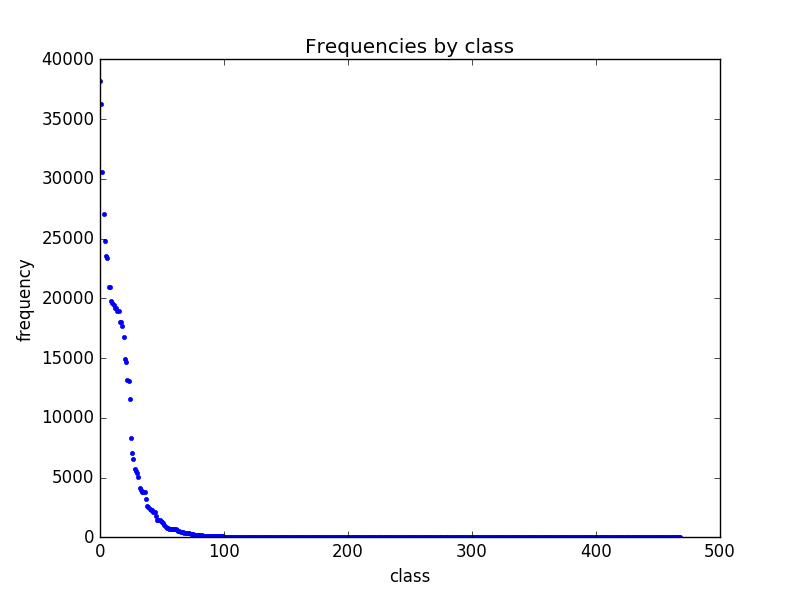
\includegraphics[width=1\textwidth]{img/dataset_frequency.png}
	\caption{Plot of frequencies for classes in \texttt{dataset}. \textit{owl:Thing} is excluded.}
	\label{fig:frequency}
\end{figure}

\section{Reasoning system}
The Stardog only interface handles the limits 
Python code for querying and using Stardog as endpoint. 
Query the dataset to calculate the in degree and out degree.

In degree takes 55 seconds, out degree takes 46 seconds.
 
\begin{lstlisting}[captionpos=b, caption=SPARQL query for calculating in degree of entities, label=lst:sparql, basicstyle=\ttfamily\small,frame=bt]
SELECT
DISTINCT ?entity
(COUNT(distinct ?pin) as ?indegree)
WHERE { 
?entity a owl:Thing .
?something ?pin ?entity .}
GROUP by ?entity
ORDER by desc(?indegree)
\end{lstlisting}

\begin{lstlisting}[captionpos=b, caption=SPARQL query for calculating out degree of entities, label=lst:sparql, basicstyle=\ttfamily\small,frame=bt]
SELECT
DISTINCT ?entity
(COUNT(distinct ?pout) as ?outdegree)
WHERE { 
?entity a owl:Thing .
?entity ?pout ?somethingelse .
}
GROUP by ?entity
ORDER by desc(?outdegree)
\end{lstlisting}

\subsection{Sub-graph extraction}
Event related graph

\subsection{Sub-graph analysis}
- new statistics

\section{Experimental set up}

\subsection{Event finding}
- Query both datasets and report on instances gotten

\section{Results and Discussion}

\section{Conclusion}
Through empirical methods, we compared the performance of two subsets of the main \texttt{dataset}. 

Weight the differences between designing an ontology or cleaning existing ontologies.

\bibliographystyle{plain}
\bibliography{mybib}

\end{document}
